\chapter{評価}
\par
行動情報と発話情報の両方を反映した心的状態の推定が有効であることを示すため,信念および欲求の推定において,MIoMと単一情報による心的状態推定システムUnimodal Inference of Mind(UIoM)を比較する.行動情報と発話情報には,本研究で作成したデータセットを利用する.

\section{実験設定}

\begin{figure}[htbp]
  \begin{center}
    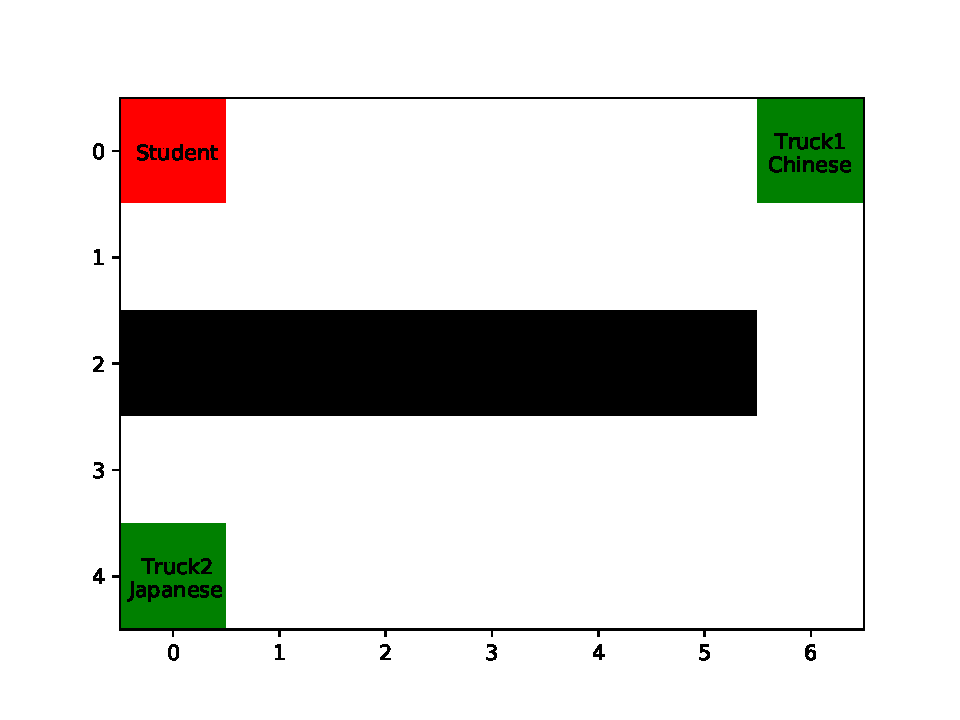
\includegraphics[]{./figure.pdf}
    \caption{本実験における環境.図中の"Student"は学生,"Truck1"および"Truck2"は屋台を開くスペース,中央の黒色部分は壁を表す.}
    \label{fig:ex_env}
  \end{center}
\end{figure}

\par
学生がアシストロボットとともに屋台で食事を買うシーンを想定する.図\ref{fig:ex_env}に本実験における環境の一例を示す.7$\times$5マスで表現される環境中に壁とTruck1およびTruck2で表される屋台を開くスペースが存在し,それぞれのスペースに日本食の屋台,イタリア料理の屋台,中華料理の屋台のいずれかが出店する.環境中の学生は移動し,アシストロボットと対話をしながら食事を購入する屋台を決める状況を考える.学生は,日本食の屋台,イタリア料理の屋台,中華料理の屋台の3種類のうち2種類が出店することは知っているが,どの屋台が出店しているかは知らないため,環境中を移動しアシストロボットと対話しながら食事を買う屋台を選ぶ.学生の行動$a_t$は上,下,左,右の4方向への移動とし,発話$u_t$はアシストロボットから提示される食事に関する質問に対する学生の応答とする.信念$b_t$は,壁により観測できていない屋台に関してどの屋台が出店していると考えているか,欲求$d$は学生が3種類のそれぞれの屋台をどの程度好むかを表す.



\section{実験手順}

\par
本実験には,本研究で作成したデータセットを利用した.本データセットには,屋台の組み合わせを表す環境設定と,その環境設定で考えられる学生の行動,アシストロボットからの質問,学生の応答が含まれる.屋台の組み合わせは日本食の屋台,イタリア料理の屋台,中華料理の屋台の2つの組み合わせとする6通り,学生の行動は上,下,左,右の4方向への移動,アシストロボットからの質問は表\ref{tab:question}に記載される4通り,学生の応答は表\ref{tab:answer}に記載される8通りである.MIoMによって行動情報と発話情報の両方を推定に活用することが有効であることを評価するために,パーティクルフィルタを用い行動情報と発話情報の一方のみを基に心的状態を推定するシステムUnimodal Inference of Mind (UIoM)を定義した.


\begin{table}[htb]
  \begin{center}
  \caption{アシストロボットからの質問と学生の応答}
  \label{tab:q_a}
  \begin{tabular}{lcc} \hline
    質問内容&\multicolumn{2}{c}{応答内容}\\\hline
    魚料理と野菜料理どちらを食べたいですか&fish&vegetable\\
    パスタと米ではどちらを食べたいですか&pasta&rice\\
    あっさりしたものと,こってりしたものどちらを食べたいですか&plain&oily\\
    辛いものと酸っぱいものではどちらを食べたいですか&spicy&sour\\\hline
  \end{tabular}
\end{center}
\end{table}



\par
30人の実験参加者に,本データセットで指定された環境設定と行動およびアシストロボットからの質問と学生の応答を提示し,環境中の学生の信念と欲求をそれぞれ7段階で推定させた.また,MIoM (action + utterance),行動情報のみを基に心的状態を推定するUIoM (action),発話情報のみを基に心的状態を推定するUIoM (utterance)の3つのシステムによって,環境中の学生の信念と欲求をそれぞれ7段階で推定した.実験参加者によって得られた推定結果とMIoMおよびUIoM によって得られた推定結果を比較し相関係数を算出した.UIoM (action)およびUIoM (utterance)の尤度は,それぞれ式(\ref{uiom_a}),式(\ref{uiom_u})で計算した.

\begin{equation}
  \begin{split}
  \label{uiom_a}
  L^k({\mathrm{action}})&= \sum_{b_{t-1}^k,o_t}P(b_t^k|b_{t-1}^k,o_t)\cdot P(o_t|s_t)\cdot P(s_t|s_{t-1},a_{t-1})\\
  &\hspace{3cm}\cdot P(a_{t-1}|b_{t-1}^k,d^k)\cdot P(b_{t-1}^k,d^k,s_{t-1},a_{t-2})
  \end{split}
\end{equation}

\begin{equation}
  \begin{split}
  \label{uiom_u}
  L^k({\mathrm{utterance}})&= \sum_{b_{t-1}^k,o_t}P(b_t^k|b_{t-1}^k,o_t)\cdot P(o_t|s_t)\cdot P(s_t|s_{t-1},a_{t-1})\\
  &\hspace{3cm}\cdot P(u_{t-1}|b_{t-1}^k,d^k)\cdot P(b_{t-1}^k,d^k,s_{t-1},u_{t-2})
  \end{split}
\end{equation}

\begin{figure}[htbp]
  \begin{center}
    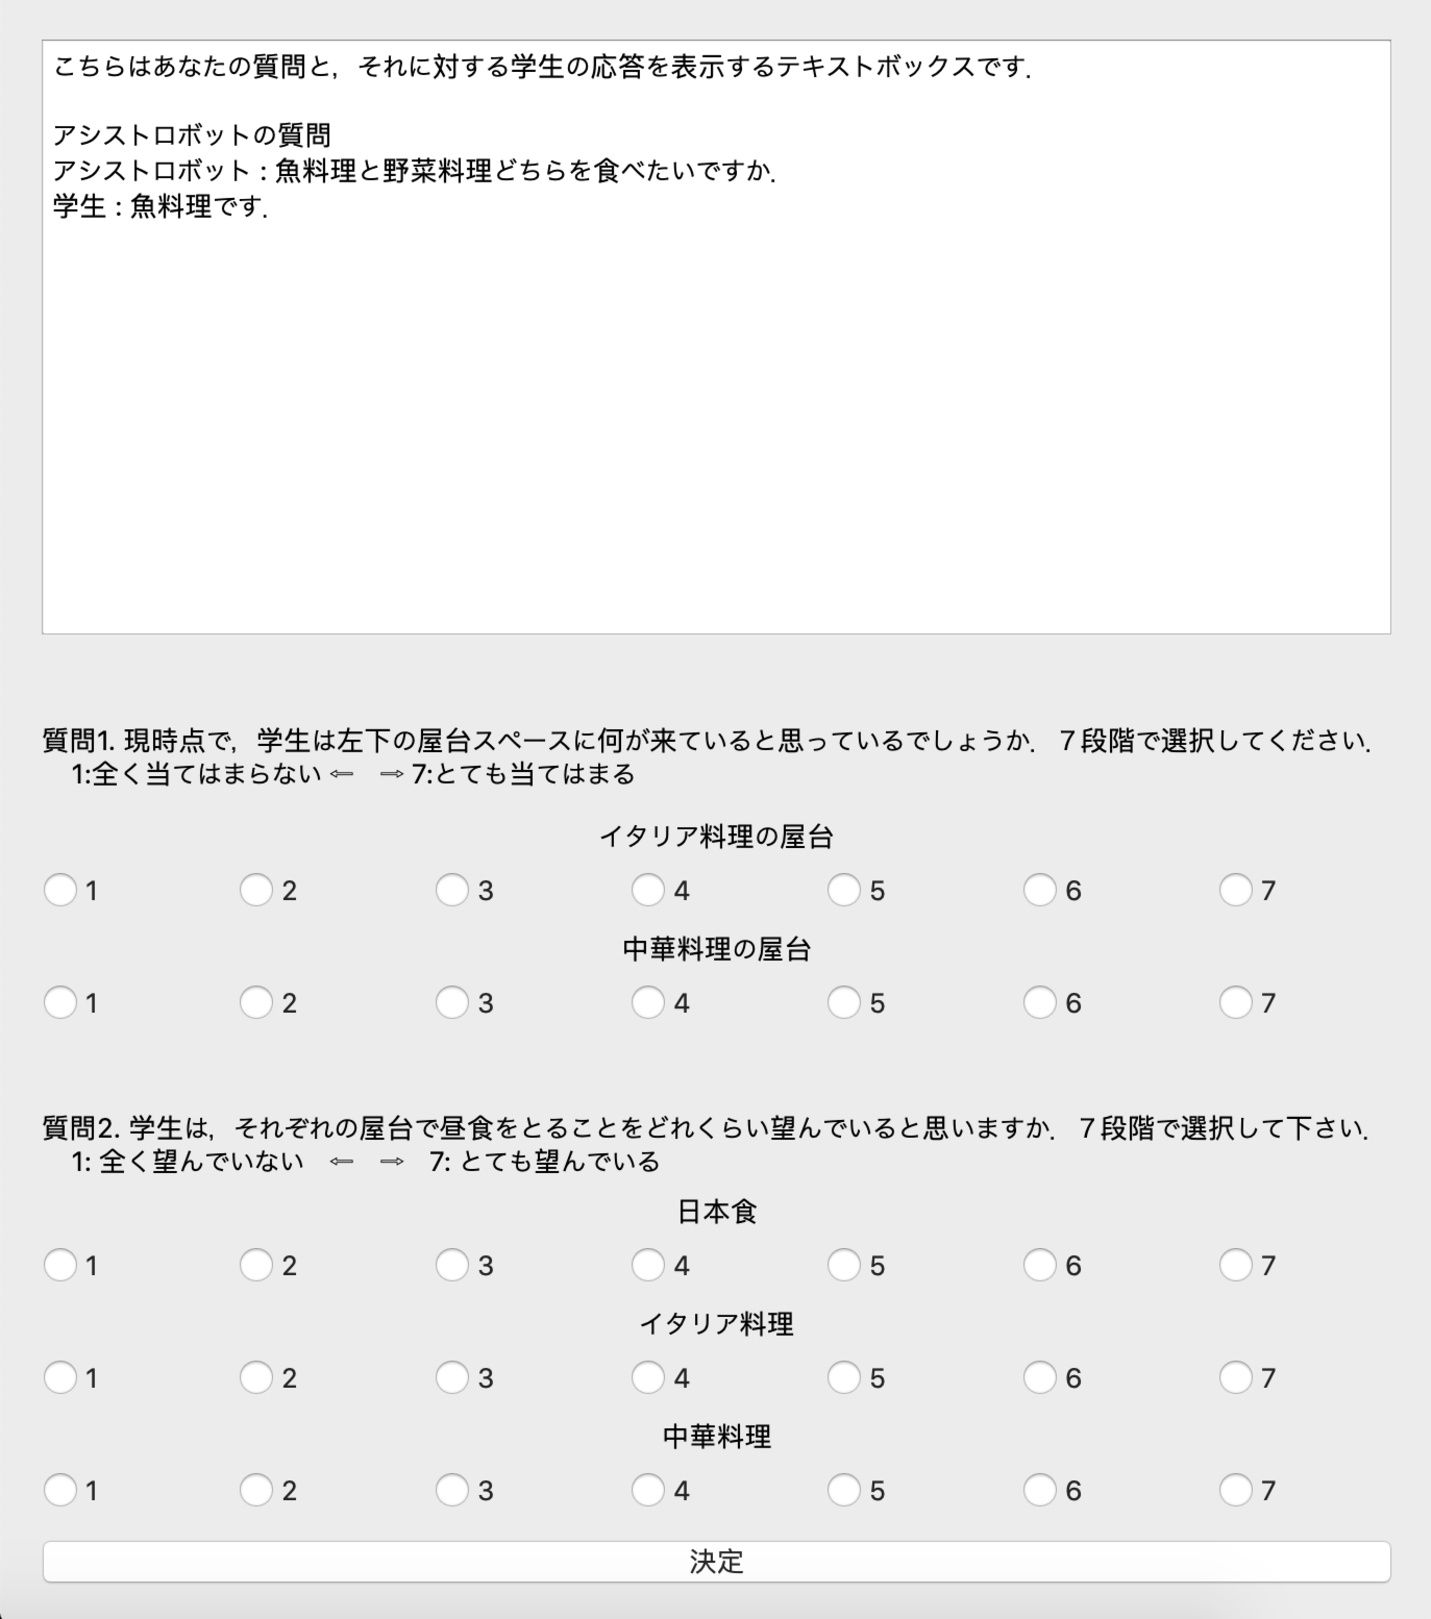
\includegraphics[scale=0.6]{./interface.pdf}
    \caption{本実験に使用したインターフェース}
    \label{fig:interface}
  \end{center}
\end{figure}

\section{実験結果}

\par
表\ref{tab:cof}に,実験参加者による信念と欲求の推定結果とUIoM (action), UIoM (utterance)およびMIoMによる信念と欲求の推定結果との間の相関係数を示す.

\begin{table}[htb]
  \begin{center}
  \caption{人間による推定と推定モデルの相関}
  \label{tab:cof}
  \begin{tabular}{lcc} \hline
    \multirow{2}{*}{モデル}&\multicolumn{2}{c}{相関}\\\cline{2-3}
    & \hspace{10pt} 信念 \hspace{10pt} & \hspace{10pt} 欲求 \hspace{10pt} \\ \hline
    UIoM (action)&0.124&0.419\\
    UIoM (utterance)&0.216&0.494\\
    MIoM (action + utterance)&\bf0.244&\bf0.549 \\\hline
  \end{tabular}
\end{center}
\end{table}


\par
表\ref{tab:cof}より,信念と欲求の推定の両方において,行動情報と発話情報の両方を推定に活用するMIoMが行動情報のみを推定に活用するUIoM (action)および発話情報のみを推定に活用するUIoM (utterance)よりも強い相関を示した.また,いずれの推定システムにおいても欲求推定の相関が信念推定の相関よりも強いことがわかった.
